\section{High-Level Overview}
 In this section we provide a high-level overview of our algorithms. First we describe our $(2+\epsilon)$-APSP algorithms for weighted graphs, by giving a simpler static version first. Then we describe our $(2+\epsilon,W_{u,v})$-APSP algorithm, where we introduce a notion of \emph{bunch overlap threshold} to overcome the challenge of dynamically maintaining a well-known static adaptive sampling technique~\cite{TZ01} (see \Cref{sc:overview2W}). 
 We give a reduction from mixed approximations to purely multiplicative approximations, which together with the previous result gives our $(2+\epsilon)$-APSP algorithm for unweighted graphs. 
Finally, we describe our $(1+\epsilon, 2(k-1))$-APSP algorithm for any $k \geq 2$ in unweighted graphs. 



\subsection{\texorpdfstring{$(2+\epsilon)$}{(2+epsilon)}-APSP for Weighted Graphs}\label{sc:high-level_2approx} 
We first present a warm-up static algorithm, that we later turn into a dynamic algorithm. 

\subsubsection{Static \texorpdfstring{$2$}{2}-APSP} 
We start by reviewing the concepts of bunch and cluster as defined in the seminal distance oracle construction of \cite{TZ2005}.

Let $0<p <1$ be a parameter and $A$ a set of nodes sampled with probability $p$. For each node $u$, the pivot $p(u)$ is the closest node in $A$ to $u$. The \textit{bunch} $B(v)$ of a node $v$ is the set $B(v):=\{ u \in V : d(u,v) < d(v,p(v)) \}$ and the \textit{clusters} are $C(u):= \{ v \in V: d(u,v) < d(v,p(v)) \}=\{v \in V: u\in B(v)\}$. Hence bunches and clusters are reverse of each other: $u \in B(v)$ if any only if $v \in C(u)$.

 These structures have been widely used in various settings, including the decremental model (e.g.~\cite{HKN2016, RodittyZ11, LN2020, Chechik18}). We can use these existing decremental algorithms to maintain bunches and clusters, but will need to develop new decremental tools to get our desired tradeoffs that we will describe in \Cref{sec:overview_dynamic}.

Using the well-known distance oracles of \cite{TZ2005}, we know that by storing the clusters and bunches and the corresponding distances inside them, we can query $3$-approximate distances for any pair. At a high-level, for querying distance between a pair $u, v$ we either have $u \in B(v)$ or $v \in B(u)$ and so we explicitly have stored their distance, or we can get a $3$-approximate estimate by computing $\min \{d(u,p(u)+d(p(u),v), d(v, p(v))+d(p(v), u)\}$. In the following we explain that in some special cases we can use these estimates to a obtain $2$-approximation for a pair $u,v$, and in other cases by storing more information depending on how $B(u)$ and $B(v)$ overlap we can also obtain a $2$-approximation to $d(u,v)$. 

Let us assume that for all nodes $v$ we have computed $B(v)$ and have access to all the distances from $v$ to each node $u \in B(v)$. Also assume that we have computed the distances from the set~$A$ to all nodes.
We now describe how using this information we can get a $2$-approximate estimate of \textit{any} pair of nodes $u,v$ in one case. In another case we will discuss what other estimates we need to precompute. Let $\pi$ be the shortest path between $u$ and $v$.
 We consider two cases depending on how the bunches $B(u)$ and $B(v)$ interact with $\pi$. A similar case analysis was used in \cite{censor2021fast, dory2022exponentially} in distributed approximate shortest paths algorithms. 
\begin{enumerate}
    \setlength\itemsep{0em}
    \item \label{overview:outside_bunch} There exists $w \in \pi$ such that $w \not \in B(u) \cup B(v)$ (left case in Figure~\ref{fig:pivots}): Since $w$ is on the shortest path, we either have $d(w,u) \leq d(u,v)/2$ or $d (v,w) \leq d(u,v)/2$. Suppose $d(w,u) \leq d(u,v)/2$. We observe that by definition $d(u,p(u))\leq d(u,w)$, hence we obtain $d(u,p(u))+d(p(u),v)\leq d(u,p(u))+d(u,p(u))+d(u,v) \leq 2d(u,v)$. The case that $d (v,w) \leq d(u,v)/2$ is analogous, and hence by computing $\min \{ d(u,p(u))+d(p(u),v), d(v,p(v))+d(p(v),u)\}$ we get a $2$-approximation.
 
    \item \label{overview:adj_bunches} There exists no $w \in \pi$ such that $w \not \in B(u) \cup B(v)$. In other words, $B(u) \cap B(v) \cap \pi = \emptyset$ and there exists at least one edge $\{u',v'\}$ on $\pi$ where $u' \in B(u)$ and $v' \in B(v)$ (right case in Figure~\ref{fig:pivots}\footnote{Although the picture implies $B(u)$ and $B(v)$ are disjoint, this also includes the case where they overlap, or even where $u\in B(v)$ or $v\in B(u)$.}): in this case we can find the minimum over estimates obtained through all such pairs $u', v'$, i.e. by computing $d(u,u')+ w(u',v')+d(v',v)$. 
\end{enumerate}

\begin{figure}[htbp!]
\centering
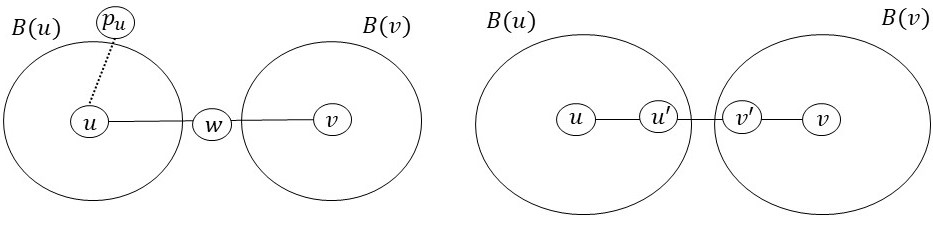
\includegraphics[width=\textwidth]{picture2}
\caption{\footnotesize Possible scenarios for the overlap between the bunches $B(u)$, $B(v)$ and the shortest path $\pi$ from $u$ to $v$.}
\label{fig:pivots}
\end{figure}    

If we had access to all the above distances for the bunches and the pivots, we could then use them to query $2$-approximate distances between any pair $u,v \in V$. As we will see, in our algorithms we only have \textit{approximate bunches and pivots} which lead to $(2+\epsilon)$-approximate queries.



\paragraph{Running time.} 
We can compute bunches and clusters in $\tilde O(\tfrac{m}{p})$ time~\cite{TZ2005}. We need to compute shortest paths from $A$ for the estimates in Case~\ref{overview:outside_bunch}. This takes $O(|A|m)=\tilde O(pnm)$ time using Dijkstra's algorithm. Finally, we consider Case~\ref{overview:adj_bunches}. A straight-forward approach is to consider each pair of vertices $u,v$, and all $u'\in B(u)$ and $v'\in B(v)$. This takes $O(\tfrac{n^2}{p^2})$ time. 

We use a sophisticated intermediate step that computes the distance between $u'$ and $v$ if there is an edge $\{u',v'\}\in E$ such that $v'\in B(v)$. For each node $v \in V$, we consider all $v'\in B(v)$, for which we consider all neighbors $u'\in N(v')$ and compute the estimate $w(u',v')+d(v',v)$ (and replace current $u'-v$ minimum if it is smaller). Since $|B(v)|=\tilde O(\tfrac{1}{p})$, we can compute these estimates for $d(u',v)$ in $\tilde O(\tfrac{n^2}{p})$ time. 

Next, for each pair $u,v\in V$, we take the minimum over the distances $d(u,u')+d(u',v)$ for all $u'$ in the bunch $B(u)$ using the precomputed distances from the previous step in time $\tilde O(n^2/p)$, by iterating over all pairs $u,v\in V$, and all $u'\in B(u)$. 
So in total the adjacent case takes time $\tilde O(\tfrac{n^2}{p})$. Hence the total running time of the algorithm will be $\tilde O(pnm+m/p+n^2/p)=\tilde O(pnm+n^2/p)$. By setting $p=\sqrt{\tfrac{n}{m}}$ we obtain the total update time $\tilde O(m^{1/2}n^{3/2})$ as stated in Theorem~\ref{thm:main_mult}, for details see \Cref{sc:mult_result}.

% Recent follow-up work in the static setting~\cite{DoryFKNVV23} that also exploits this trick shows how to compute Case~\ref{overview:adj_bunches} in $\tilde O(\tfrac{m}{p^2})$ time, obtaining a total running time of $\tilde O(mn^{2/3})$. \ttodo{keep or delete this sentence? I think our story changed a bit and we could take it out.} \mtodo{yes, not sure that it's needed here}

There are several subtleties that make it more difficult to maintain these estimates in decremental settings since the bunches and which bunches are adjacent keep on changing over the updates. We next discuss how these can be handled. We obtain a total update time that matches the stated static running time (up to subpolynomial factors). %for the algorithm using bunch overlap thresholds. \mtodo{removed this, seems that it stayed from a previous version}

    
\subsubsection{Dynamic Challenges}\label{sec:overview_dynamic}
\paragraph{Maintaining bunches and pivots.}
First, we need to dynamically maintain bunches efficiently as nodes may join and leave a bunch throughout the updates using an adaptation of prior work. One option would be maintaining the clusters and bunches using the \cite{RZ12} framework, however using this directly is slow for our purposes. Hence we maintain \textit{approximate} clusters and bunches using hopsets of \cite{LN2020}. This algorithm also maintains approximate pivots, i.e.~pivots that are within $(1+\epsilon)$-approximate distance of the true closest sampled node. These estimates let us handle the first case (up to $(1+\epsilon)$ approximation).
One subtlety is that the type of approximate bunches used in \cite{LN2020} is slightly different with the type of approximate bunches we need for other parts of our algorithm. Specifically we need to bound the number of times nodes in a bunch can change. Roughly speaking, we can show this since the graph is decremental and the estimates obtained from the algorithm of \cite{LN2020} are monotone. Hence we perform \emph{lazy bunch updates}, where we only let a bunch grow if the distance to the pivot grows by at least a factor $1+\epsilon$. This means a bunch grows at most $O(\log_{1+\epsilon}(nW))$ times. In addition, these approximate bunches need to be taken into account into our stretch analysis. 

We note that $(1+\epsilon)$-approximate decremental SSSP takes $\tilde O(m^{1+o(1)})$ total update time. However, we use the multi-source shortest path result from~\cite{LN2020}, where the $n^{o(1)}$-term vanishes when applied with polynomially many sources, giving us a total update time of $\tilde O(|A|m)$.
 

\paragraph{Maintaining estimates for Case~\ref{overview:adj_bunches}.}
When we are in Case~\ref{overview:adj_bunches}, we need more tools to keep track of estimates going through these nodes since both the bunches and the distances involved are changing. In particular, we explain how by using heaps in different parts of our algorithm we get efficient update and query times.
Moreover, note that we have an additional complication: there are two data structures in this step, where one impacts the other. We need to ensure that an update in the original graph does not lead to many changes in the first data structure, which all need to be processed for the second data structure. 

To be precise, we need intermediate data structures $Q_{u',v}$ that store approximate distances for $u'$ and $v$ of the form $w(u',v')+\delta(v',v)$ for each $v'\in B(v)$ such that $\{u',v'\}\in E$, as explained for the static algorithm\footnote{In this section, $\delta(\cdot,\cdot)$ denotes $(1+\epsilon)$-approximate distances in our dynamic data structures.}. As opposed to the static algorithm, we do not only keep the minimum, but instead maintain a min-heap, from which the minimum is easily extracted. 

However, this approach has a problem: $\delta(v',v)$ might change many times, and for each such change we need to update at most $|N(v')|\leq n$ heaps. To overcome this problem, we use another notion of \textit{lazy distance update}: we only update a bunch if the estimate of a node changes by at least a factor $1+\epsilon$. Combining this with the fact that, due to the lazy \textit{bunch} update, nodes only join a cluster at most $O(\log_{1+\epsilon}(nW))$ times, and thus there is only an $ O(\log_{1+\epsilon}(nW)\log(nW))$ overhead in maintaining these min-heaps $Q_{u',v}$ dynamically due to bunch updates. 

Similarly, $w(u',v')$ might change many times, which has an impact for every $v\in C(v')$. Since this can be many nodes, we need to use an additional trick so an adversary cannot increase our update time to $mn$. Again the solution is a lazy update scheme: instead of $w(u',v')$ we use $\tilde w(u', v')=(1+\epsilon)^{\lceil \log_{1+\epsilon} w(u',v')\rceil}$, which can only change $\log_{1+\epsilon} W$ times. This comes at the cost of a $(1+\epsilon)$ approximation factor. 


We note that our bunches are approximate bunches in three different ways. We have one notion of approximation due to the fact that we are using hopsets (that implicitly maintain bunches on scaled graphs). We have a second notion of approximation due to our lazy bunch update, which only lets nodes join a bunch a bounded number of times. We have a third notion of approximation due to the lazy distance update, which only propagates distance changes $O(\log(nW))$ times. We need to carefully consider how these different notions of approximate bunch interact with each other and with the stretch of the algorithm.

Next, we want to use the min-heaps $Q_{u',v}$ to maintain the distance estimates for $u,v\in V$ (see again the right case in Figure~\ref{fig:pivots}). We construct min-heaps $Q'_{u,v}$, with for each pair $u,v$ entries $\delta(u,u')+\delta(u',v)$ for $u' \in B(u)$. Here $\delta(u',v)$ is the minimum from the intermediate data structure $Q_{u',v}$. 

An entry $\delta(u,u')+\delta(u',v)$ in $Q'_{u,v}$ has to be updated when either $\delta(u,u')$ or $\delta(u',v)$ change. We have to make sure we do not have to update these entries too often. For the first part of each entry, we bound updates to the distance estimates $\delta(u,u')$ by the lazy distance updates. One challenge here is that when the distance estimates in a bunch change we need to update all the impacted heaps i.e.~if $\delta(u,u')$ inside a bunch $B(u)$ changes, we must update all the heaps $Q'_{u,v}$ such that there exists $\{u',v'\} \in E$ with $v'\in B(v)$. For this purpose one approach is the following: for each $u \in V,u' \in B(u)$ we keep an additional data structure $\text{Set}_{u,u'}$ that stores for which $v \in V$ we have $v' \in B(v)$ with $\{u',v'\}\in E$. This means that given a change in $\delta(u,u')$, we can update each of the heaps in logarithmic time. 


For the second part of the entry, which is the distance estimate $\delta(u',v)$ from the first data structure, this is more complicated. Another subtlety for our decremental data structures is the fact that $\delta(u',v)$ may also \text{decrease} due to a new node being added to $B(v)$. However, our lazy bunch update ensures that $\delta(u',v)$ can only decrease $O(\log_{1+\epsilon}(nW))$ times. Further, we use lazy distance increases \textit{in between} such decreases. Hence in total we propagate changes to $\delta(u',v)$ at most $O(\log_{1+\epsilon}(nW)\log(nW))$ times, and thus our decremental algorithm has $\tilde O(\log_{1+\epsilon}(nW)\log(nW))$ overhead compared to the static algorithm.

\subsection{\texorpdfstring{$(2+\epsilon, W_{u,v})$}{(2+epsilon,W{u,v})}-APSP for Weighted Graphs}\label{sc:overview2W}
For a moment, let us go back to the first static algorithm. It turns out, that if instead of computing an estimate for two `adjacent' bunches, we keep an estimate for bunches that overlap in at least one node, we obtain a $(2, W_{u,v})$-approximation, where $W_{u,v}$ is the maximum weight on the shortest path from $u$ to $v$. 

\begin{figure}[htbp!]
    \centering
    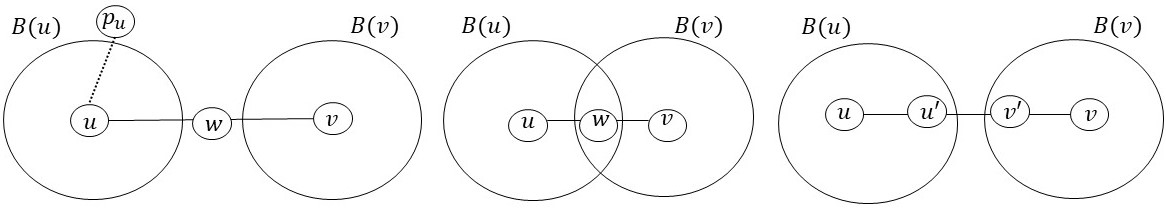
\includegraphics[width=\textwidth]{picture_new}
    \caption{Possible scenarios for the overlap between the bunches $B(u)$ and $B(v)$ and the shortest path $\pi$ from $u$ to $v$.}
    \label{fig:pivots_allcases_overview}
\end{figure}

The stretch analysis comes down to the following cases:
\begin{itemize}%\setcounter{enumi}{2}
    \item There exists no $w\in \pi\cap B(u)\cap B(v)$ (the left and right case in \Cref{fig:pivots_allcases_overview}). 
    \item There exists $w\in \pi$ such that $w\in B(u)\cap B(v)$ (the middle case in \Cref{fig:pivots_allcases_overview}). \label{overview:overlap}
\end{itemize}

The crucial observation here is that the distance estimate via the pivot (Case~\ref{overview:outside_bunch} in the previous section) already gives a $(2, W_{u,v})$-approximation for the adjacent case (the right case in \Cref{fig:pivots_allcases_overview}), see \Cref{sec:2_W} for the details. So if we maintain an estimate for $d(u,v)$ if there exists $w\in \pi$ such that $w\in B(u)\cap B(v)$ (the `overlap case'), then we obtain a $(2, W_{u,v})$-approximation in total. 


Here we need to create a min-heap for the overlap case, later we show we can maintain in $\tilde O(nC_{\max}/p)$ time. First we focus on the challenge of bounding $C_{\max}$.

\paragraph{Efficiency challenge.}
While the bunches are small, there is no bound on the size of the clusters. To overcome this issue in the static case, Thorup and Zwick developed an alternative way to build the bunches and clusters, that guarantees that the clusters are also small \cite{TZ01}. At a high-level, their approach is to adaptively change (grow) $A$ by sampling big clusters into smaller clusters using a sampling rate proportional to the cluster size and adding these nodes to the set of pivots $A$. In total, in $\tilde O(m/p)$ time we obtain bunches and clusters, \emph{both} of size $\tilde O(1/p)$.
This idea was developed in the context of obtaining compact routing schemes, and later found numerous applications in static algorithms for approximating shortest paths and distances (see e.g., \cite{BaswanaK10,AkavR20,backurs2021toward,AkavR21}).

Using this trick, the static algorithm has running time $\tilde {O}(\tfrac{m}{p}+pnm+\tfrac{n}{p^2})=\tilde O(nm^{3/4}+m^{4/3})$, for $p=m^{-1/3}$ or $\tilde O(mn^{1/2}+n^2)$ for $p=n^{-1/2}$. 


However, the adaptive sampling procedure does not seem to be well-suited to a dynamic setting. The reason is that the sampling procedure is adaptive in such a way that when the bunches/clusters change, the set of sampled nodes can also change. Although (a dynamic adaptation of) the algorithm can guarantee that the set of sampled nodes is small at any particular moment, there is no guarantee on the \emph{monotonicity} of the set $A$ of sources that we need to maintain distances from. This would add a significant amount of computation necessary to propagate these changes to other parts of the algorithm. A possible solution is to enforce monotonicity by never letting nodes leave $A$. This would require us to bound the \emph{total} number of nodes that would ever be sampled, which seems impossible with the current approach. 
To overcome this, we next suggest a new approach that gives us the monotonicity needed for our dynamic algorithm. For simplicity, we first present this in a static setting. 


% \mtodo{it's not ideal that this part which may be the most interesting on a technical level appears now towards the end of the overview, I wonder if it makes sense to change the order a bit, either discuss first the $(2,W)$-approximation, or move the subsection about dynamic challenges to a later place after we discuss both algorithms? (start with the static version, and then go to the dynamic ones, not sure if it makes sense)}

\paragraph{Introducing bunch overlap thresholds.} Our proposed approach is to divide the nodes into two types depending on the number of bunches they appear in.
In particular, we consider a threshold parameter $\tau$ and we define a node to be a \textit{heavy node} if it is in more than $\tau$ bunches (equivalently its cluster contains more than $ \tau $ nodes), and otherwise we call it a \textit{light node}. In other words, for the set of light nodes we have $C_{\max}\leq \tau$. This threshold introduces a second type of pivot for each node $u$, which we denote by $q(u)$ that is defined to be the closest heavy node to $u$. In particular, instead of computing all distance estimates going through nodes $w \in B(u) \cap B(v)$, we only compute them for the case that $w$ is light, and otherwise it is enough to compute the minimum estimates going through the heavy pivots, i.e.~$\min \{ d(u,q(u))+d(q(u),v), d(v,q(v))+d(q(v),u)\}$. We emphasize that these heavy pivots are \textit{not a subset} of our original pivots $p(v), v \in V$, and they have a different behavior in bounding the running time than the \textit{bunch pivots}.
 As we will see later, introducing these thresholds is crucial in efficiently obtaining the estimates required for Case~\ref{overview:overlap} as we can handle the light and heavy case separately.


\paragraph{Stretch of the algorithm with bunch overlap thresholds.} As discussed above, the stretch analysis was divided into two cases. In the new variant of the algorithm we add a third case, where we look at the distance estimates going through heavy pivots, i.e.~$\min \{ d(u,q(u))+d(q(u),v), d(v,q(v))+d(q(v),u)\}$. The main idea is that now we only need to consider the difficult case, Case~\ref{overview:overlap}, if the relevant node is light, which allows us to implement the algorithm efficiently. 

If the relevant node $w\in B(u)\cap B(v)$ in Case~\ref{overview:adj_bunches} is heavy, we obtain a 2-approximation through the heavy pivot: we get that the $\min\{d(u,w),d(v,w)\} \leq d(u,v)/2$, since $d(u,v)= d(u,w)+d(w,v)$. W.l.o.g.\ say $d(u,w)\leq d(u,v)/2$. Then $d(u,q(u))\leq d(u,w)\leq d(u,v)/2$, hence $d(u,q(u))+d(q(u),v)\leq d(u,q(u))+d(q(u),u)+d(u,v) \leq 2d(u,v)$. 

\paragraph{Maintaining estimates through heavy nodes.}
For the stretch analysis above, we need to maintain a shortest path tree from each heavy node. We ensure a bunch grows at most $O(\log_{1+\epsilon}(nW))$ times. Hence by a total load argument we get that the \emph{total} number of nodes in all bunches over all updates is at most $O(\tfrac{n}{p}\log_{1+\epsilon}(nW))$. This implies there cannot be too many heavy nodes in total, hence we can enforce monotonicity by keeping in $V_{\rm{heavy}}$ all nodes that were once heavy (for details see Lemma~\ref{lm:size_heavy}). As a consequence, we can maintain multi-source approximate distances from all heavy nodes efficiently: we can compute shortest paths from this set to all other nodes in $O(|V_{\rm{heavy}}|m)=O(\tfrac{nm}{p\tau})$ time.


\paragraph{Running time of the algorithm with bunch overlap thresholds.}
Summarizing, we compute bunches and clusters in $O(m/p)$ time, compute distances from $A$ to $V$ in $O(|A|m)=\tilde O(pnm)$ time, and we can compute shortest paths from ththe heavy nodes in $O(|V_{\rm{heavy}}|m)=O(\tfrac{nm}{p\tau})$ time.


Finally, we consider Case~\ref{overview:overlap}. For each node $u\in V$, we consider every light node $w\in B(u)$, and then all nodes $v\in C(W)$. Since $w$ is light, we have $|C(w)|\leq \tau$, so this takes time $\tilde O(n\cdot \tfrac{1}{p}\cdot \tau)$.  

Hence, in the total update time, we obtain $\tilde O((pnm+\tfrac{nm}{p\tau}+n\tau/p)\log^2(nW))$. Setting $p=m^{-1/4}$ and $\tau = m^{1/2}$ gives a total update time of $\tilde O(nm^{3/4}\log(nW))$. We provide the details in \Cref{sc:2_W}.

Again for a decremental algorithm, we need to combine this new idea with the subtleties we had in the previous section: the bunches, their overlaps, and the heavy nodes keep on changing over the updates. We obtain a total update time that matches the stated static running time (up to subpolynomial factors) for the algorithm using bunch overlap thresholds. 

 





\subsubsection{\texorpdfstring{$(2+\epsilon)$}{(2+epsilon)}-APSP for Unweighted Graphs} 
We observe that in unweighted graphs mixed approximation can always be turned into a multiplicative approximation -- at the cost of a blow-up in the number of vertices. More precisely, we prove the following reduction. 
\begin{restatable}{theorem}{thmreduction}\label{thm:reduction}
   Let $\mathcal A$ be an algorithm that provides a $(a+\epsilon,k)$-approximation for APSP in $\tau_{\mathcal A}(n',m')$ time, for any unweighted $n'$-node $m'$-edge graph $G'$, and any constants  $a,k\in \mathbb N_{\geq 1}$ and $\epsilon\in[0,1)$. Given an unweighted graph $G=(V,E)$ on $n$ nodes and $m$ vertices, we can compute $(a+(k+2)\epsilon,0)$-APSP in $\tau_{\mathcal A}(n+km,(k+1)m)$ time. 

    If $\mathcal A$ is a dynamic algorithm, then each update takes $(k+1)\cdot [\text{update time of }\mathcal A]$ time. The query time remains the same (up to a constant factor). 
\end{restatable}
The result is obtained by splitting every edge into $k$ edges, by introducing new nodes on the edge. Now a path corresponding to a $+k$ approximation cannot take a non-trivial detour. 

We combine this result with \Cref{thm:(2_1)approx} to obtain a $(2+\epsilon)$-approximation for unweighted graphs in $\tilde O(m^{7/4})$ total update time. For details, see \Cref{sec:reduction}.




\subsection{\texorpdfstring{$(1+\epsilon, 2(k-1))$}{(1+epsilon,2(k-1))}-APSP for Unweighted Graphs} \label{sec:add_overview}

%In this section, we describe our decremental $(1+\epsilon,2(k-1))$-approximate APSP algorithms, that take $O(n^{2-1/k+o(1)}m^{1/k})$ total update time in unweighted graphs.

In this section, we describe our near-additive APSP algorithm.
%\paragraph{Our approach.} To overcome the above issues, we use a different approach. 
Our work is inspired by a classic result of Dor, Halperin, and Zwick \cite{DHZ00}, that presented a static algorithm that computes purely additive $+2(k-1)$ approximation for APSP in $\tilde{O}(n^{2-1/k}m^{1/k})$ time in unweighted graphs. Our goal is to obtain similar results dynamically. 
More concretely, we obtain decremental $(1+\epsilon,2(k-1))$-approximate APSP in $O(n^{2-1/k+o(1)}m^{1/k})$ total update time in unweighted graphs.

\subsubsection{\texorpdfstring{$\mathbf{(1+\epsilon,2)}$}{(1+epsilon)}-APSP}
To explain the high-level idea of the algorithm, we first focus on the special case that $k=2$, and that we only want to approximate the distances between pairs of nodes at distance at most $d$ from each other, for a parameter $d$. In this case, we obtain a $+2$-additive approximation in $\tilde{O}(n^{3/2}m^{1/2} d )$ time. This case already allows to present many of the high-level ideas of the algorithm. Later we explain how to extend the results to the more general case.
 We start by describing the static algorithm from \cite{DHZ00}, and then explain the dynamic version. 
The static version of the data structure is as follows:

\begin{itemize}
    \setlength\itemsep{0em}
    \item Let $s_1= (\frac{m}{n})^{1/2}$. Let $V_1$ be the set of \textit{dense nodes}: $V_1:= \{ v \in V: \deg(v) \geq s_1\}$. Also let $E_2$ be the set of \textit{sparse edges}, i.e. edges with at least one endpoint with degree less than $s_1$.
    \item \textbf{Node set $D_1$.} Construct a hitting set $D_1$ of nodes in $V_1$. %by adding each node to $D_1$ with probability $\frac{c\ln{n}}{d_1}$ for a constant $c \geq 2$ for our choice. 
    This means that every node $v \in V_1$ has a neighbor in $D_1$. The size of $D_1$ is $O(n \log{n}/s_1)$.
    \item \textbf{Edge set $E^*$.} Let $E^*$ be a set of size $O(n)$ such that for each $v \in V_1$, there exists $u \in D_1 \cap N(v)$ such that $\{u,v\} \in E^*$.
    \item \textbf{Computing distances from $D_1$.} Store distances $D_1 \times V$ by running a BFS from each $u \in D_1$ on the input graph $G$. 
    \item \textbf{Computing distances from $V \setminus D_1$. } For each $u \in V \setminus D_1$ store a shortest path tree, denoted by $T_u$  rooted at $u$ by running Dijkstra on $(V, E_2 \cup E^* \cup E^{D_1}_u)$, where $E^{D_1}_u$ is the set of weighted edges corresponding to distances in $(\{u\} \times D_1)$ computed in the previous step. 
\end{itemize}

\paragraph{Dynamic data structure.} 
The static algorithm computes distances in two steps. First, it computes distances from $D_1$ by computing BFS trees in the graph $G$. This step can be maintained dynamically by using \emph{Even-Shiloach trees (ES-trees)} \cite{ES81}, a data structure that maintains distances in a decremental graph. Maintaining the distances up to distance $O(d)$ takes $O(|D_1|md)$ time.
The more challenging part is computing distances from $V \setminus D_1$. Here the static algorithm computes distances in the graphs $H_u=(V, E_2 \cup E^* \cup E^{D_1}_u)$. Note that the graphs $H_u$ change dynamically in several ways. First, in the static algorithm, the set $E_2$ is the set of light edges. To keep the correctness of the dynamic algorithm, every time that a node $v$ no longer has a neighbor in $D_1$, we should add all its adjacent edges to $E_2$. Second, when an edge in $E^*$ is deleted from $G$, we should replace it by an alternative edge if such an edge exists. Finally, the weights of the edges in $E^{D_1}_u$ can change over time, when the estimates change. This means that other than deletions of edges, we can also add new edges to the graphs $H_u$ or change the weights of their edges. Because of these edge insertions we can no longer use the standard ES-tree data structure to maintain the distances, because that only works in a decremental setting. 

To overcome this, we use \emph{monotone ES-trees}, a generalization of ES-trees proposed by \cite{HKN2016,HKN14}. In this data structure, to keep the algorithm efficient, when new edges are inserted, the distance estimates do not change. In particular, when edges are inserted, some distances may decrease, however, in such cases the data structure keeps an old larger estimate of the distance. The main challenge in using this data structure is to show that the stretch analysis still holds. In particular, in our case, the stretch analysis of the static algorithm was based on the fact the distances from the nodes $V \setminus D_1$ are computed in the graphs $H_u$, where in the dynamic setting, we do not have this guarantee anymore.  

\paragraph{Stretch analysis.}

The high-level idea of the stretch analysis uses the special structure of the graphs $H_u$. To prove that the distance estimate between $u$ and $v$ is at most $d(u,v)+2$, we distinguish between two cases. First, we maintain the property that as long as $v$ has a neighbor $x \in D_1$, then an edge of the form $\{v,x\}$ is in $E^*$ for $x \in D_1 \cap N(v)$, and since we maintain correctly the distances from $D_1$, we can prove that we get an additive stretch of at most 2 in this case. 

In the second case, all the edges adjacent to $v$ are in $E_2 \subseteq H_u$, and here we can use an inductive argument on the length of the path to prove that we get an additive stretch of at most 2. Note that the estimate that we get can be larger compared to the distance between $u$ and $v$ in the graph $H_u$, but we can still show that the additive approximation is at most 2 as needed. For a detailed stretch analysis, see \Cref{sec:add_warmup_stretch}.

\paragraph{Update time.}

Our update time depends on the size of the graphs $H_u$. While in the static setting it is easy to bound the number of edges in $E_2$ and $E^*$, in the decremental setting, as new edges are added to these sets, we need a more careful analysis. For example, in the static setting $|E^*|=O(n)$, as any node only adds one adjacent edge to the set $E^*$, where in the decremental setting, we may need to add many different edges to this set because the previous ones got deleted. However, we can still prove that even if a node needs to add to $E^*$ edges to all its adjacent neighbors in $D_1$ during the algorithm, the size of $H_u$ is small enough as needed. A detailed analysis of the update time appears in \Cref{sec:warmup_add_time}, where we show that the total update time is $\tilde{O}(m^{1/2}n^{3/2}d)$ in expectation, this matches the static complexity up to the factor $d$.

\paragraph{Handling large distances.} The algorithm described above is efficient if $d$ is small, to obtain an efficient algorithm for the general case, we combine our approach with a decremental near-additive APSP algorithm. More concretely, we use an algorithm from \cite{HKN14} that allows to compute $(1+\epsilon,\beta)$-approximation for APSP in $O(n^{2+o(1)})$ total update time, for $\beta=n^{o(1)}$. Now we set $d=\Theta(\beta/\epsilon)$, and distinguish between two cases. For pairs of nodes at distance at most $d$ from each other, we get a $+2$-additive approximation as discussed above, in $O(m^{1/2}n^{3/2+o(1)})$ time. For pairs of nodes at distance larger than $d$, the near-additive approximation is already a $(1+O(\epsilon))$-approximation by the choice of the parameter $d$. For such pairs, the additive $\beta$ term becomes negligible, as their distance is $\Omega(\beta/\epsilon)$. 
Overall, we get a $(1+\epsilon,2)$-approximation for APSP in $O(m^{1/2}n^{3/2+o(1)})$ time. In fact, if the graph is dense enough ($m=n^{1+\Omega(1)}$), the $n^{o(1)}$ term is replaced by a poly-logarithmic term. For more details see \Cref{sec_summary_additive}. 

\subsubsection{General \texorpdfstring{$k$}{k}}
We can extend the algorithm to obtain a $(1+\epsilon,2(k-1))$-approximate APSP in $O(n^{2-1/k+o(1)}m^{1/k})$ total update time, by adapting the general algorithm of \cite{DHZ00} to the dynamic setting.
At a high-level, instead of having one hitting set $D_1$, we have a series of hitting sets $D_1,D_2,...,D_k$, such that the set $D_i$ hits nodes of degree $s_i$. We compute distances from $D_i$ in appropriate graphs $H_u^i$, that are sparser when the set $D_i$ is larger. Balancing the parameters of the algorithm leads to the desired total update time. For full details and proofs see \Cref{sec:add_general}.
%\sebastian{Maybe we could add some short explanation that the whole complexity of the monotone ES-tree argument is already seen in the +2 case.}

\subsubsection{Limitations of previous approaches} 
We next explain why approaches used in previous decremental algorithms cannot be generalized to obtain our near-additive results. First, the unweighted $(1+\epsilon,2)$-approximate APSP algorithm that takes $\tilde{O}(n^{5/2}/\epsilon)$ time \cite{HKN2016}, is inspired by static algorithms for $+2$-additive emulators, sparse graphs that preserve the distances up to a $+2$-additive stretch. The main idea is to maintain a sparse emulator of size $\tilde{O}(n^{3/2})$, and exploit its sparsity to obtain a fast algorithm. This construction however is specific for the $+2$ case, and cannot be generalized to a general $k$. Note that the update time of the algorithm crucially depends on the size of the emulator, and to obtain a better algorithm for a general $k$, we need to be able to construct a sparser emulator for a general $k$.
However, a beautiful lower bound result by Abboud and Bodwin \cite{abboud20174} shows that for any constant $k$, a purely additive $+k$ emulator should have $\Omega(n^{4/3-\epsilon})$ edges. 
This implies that dynamic algorithms that are based on purely additive emulators seem to require $\Omega(n^{7/3-\epsilon})$ time, and we cannot get running time arbitrarily close to $O(n^2)$. An alternative approach is to build a \emph{near-additive} emulator. This is done in \cite{HKN14}, where the authors show a $(1+\epsilon, 2(1+2/\epsilon)^{k-2})$-approximation algorithm for decremental APSP with expected total update time of $\tilde{O}(n^{2+1/k} (37/\epsilon)^{k-1})$. Here the running time indeed gets closer to $O(n^2)$, but this comes at a price of a much worse additive term of $2(1+2/\epsilon)^{k-2}$. While in the static setting there are also other bounds obtained for near-additive emulators, such as $O(1+\epsilon,O(k/\epsilon)^{k-1})$ emulators of size $O(kn^{1+\frac{1}{2^{k+1}-1}})$ \cite{elkin2004,thorup2006spanners,abboud2018hierarchy,elkin2020near}, in all of the constructions the additive term depends on $\epsilon$, and the dependence on $\epsilon$ is known to be nearly tight for small $k$ by lower bounds from \cite{abboud2018hierarchy}. Hence this approach cannot lead to small constant additive terms that do not depend on $\epsilon$.


\paragraph{Outline.}
The detailed description of our $(2+\epsilon)$-APSP algorithms for weighted graphs can be found in \Cref{sec:TZ_2+eps}. In \Cref{sc:2_W}, we provide the algorithm for $(2+\epsilon,W_{u,v})$-APSP. In \Cref{sec:reduction}, we provide our reduction for purely multiplicative APSP and the result for $(2+\epsilon)$-APSP for unweighted graphs. And finally in \Cref{sc:additive}, we describe our $(1+\epsilon, 2(k-1))$-APSP algorithm for any $k \geq 2$ in unweighted graphs. 
